Der grundsätzliche Aufbau besteht aus einem auf einer Schiene beweglichem Wagen, welcher durch einen Motor auf dieser bewegt werden kann, sowie einem fest ausgerichtetem Mikrofon, auf welches sich der Wagen zu- bzw. wegbewegen kann.
\subsection{Messung der Wagengeschwindigkeit}
Zunächst wird die Geschwindigkeit $v$ des Wagens für alle vorhandenen Gänge gemessen, denn diese ist wichtig zur Bestimmung des Doppler-Effekts in Abhängigkeit der Quellengeschwindigkeit. Dies geschieht mit dem in Abb. 1 gezeigten Aufbaus. Die beiden angebrachten Lichtschranken registrieren das Durchfahren des Wagens, damit lässt sich die eingezeichnete Strecke $S$ messen.
\subsection{Messung der Schallgeschwindigkeit c}
Der schematische Aufbau zur Messung der Schallgeschwindigkeit wird in Abb. 2 wiedergegeben. Die am Mikrofon gemessenen und die am Frequenzgenerator erzeugten Signale werden auf ein Oszilloskop gegeben, wodurch sich Lissajous-Figuren betrachten lassen. Nun wird mit Hilfe der Lissajous-Figuren die Wellenlänge gemessen und mit dem entsprechenden Abstand lässt sich daraus die Schallgeschwindigkeit bestimmen. 
\subsection{Messung der Frequenz}
Zuerst wird die Frequenz einer ruhenden Quelle gemessen, danach die Frequenz bei bewegter Quelle für verschiedene Geschwindigkeiten. Die Messungen werden mit dem selben Aufbau durchgeführt.
Die Messung der Frequenz bei bewegter Quelle hat nur einen kleinen Effekt. Aus diesem Grund wird die in Abb. 3 angegebene Schaltung benutzt.
Die Schallquelle wird nun auf den Empfänger zu- und von ihm
wegbewegt, wobei eine Lichtschranke passiert wird und damit der Zählvorgang
auslöst wird. Die Zeitbasis steuert die Länge des Zählvorgangs, der Untersetzungsfaktor wird hier auf $10^6$ gestellt.
\subsection{Messung der Frequenzdifferenz mittels Schwebung}
Die Schaltung ändert sich nur geringfügig (s. Abb. 4), allerdings steht die Schallquelle nun fest neben dem Mikrofon und auf dem Wagen wird ein Schallreflektor befestigt. \\
Das Mikrofon registriert sowohl das Ruhe- als auch das verschobene Signal, da dies für die Messung sehr ungünstig ist, wird noch ein Tiefpass zwischen geschaltet, der die Frequenzdifferenz $\Delta\nu$ heraus filtert und zwar zu den Bedingungen:
\begin{equation*}
2\pi\nu_0 RC \gg 1
\end{equation*}
und
\begin{equation*}
2\pi\Delta\nu RC \ll 1
\end{equation*}
\subsection{Schematischer Aufbau für verschiedener Versuchsteile}
\begin{figure}[!h]
  \centering
  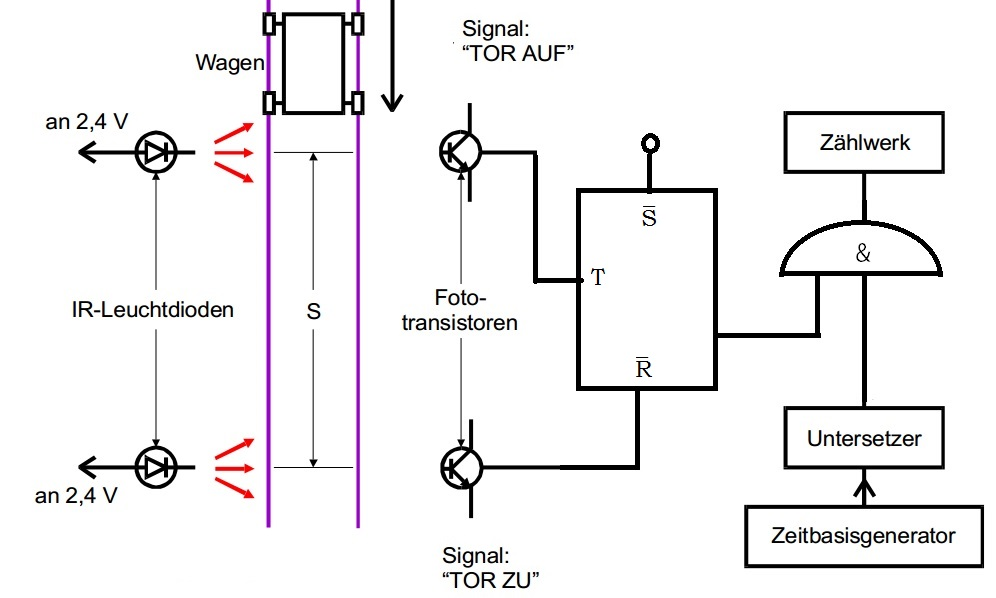
\includegraphics[scale=0.5]{Grafiken/V104_Abb1.jpg}
  \caption{Aufbau für die Messung der Wagengeschwindigkeit (verändert aus \cite{V104})}
  \label{fig:V104_Abb1}
\end{figure}
\begin{figure}[!h]
  \centering
  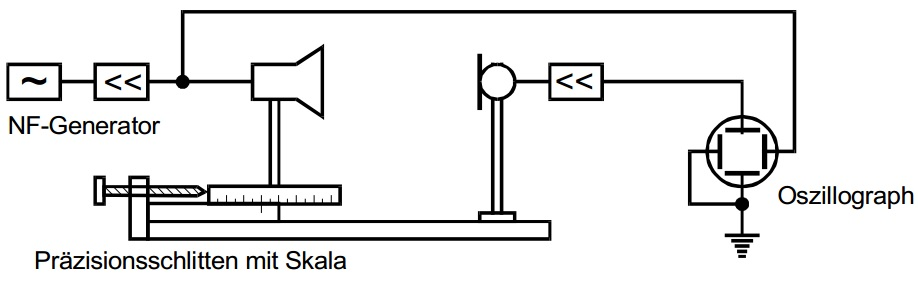
\includegraphics[width=1\textwidth]{Grafiken/V104_Abb2.jpg}
  \caption{Aufbau für die Messung der Schallgeschwindigkeit c  \cite{V104}}
  \label{fig:V104_Abb2}
\end{figure}
\begin{figure}[!h]
  \centering
  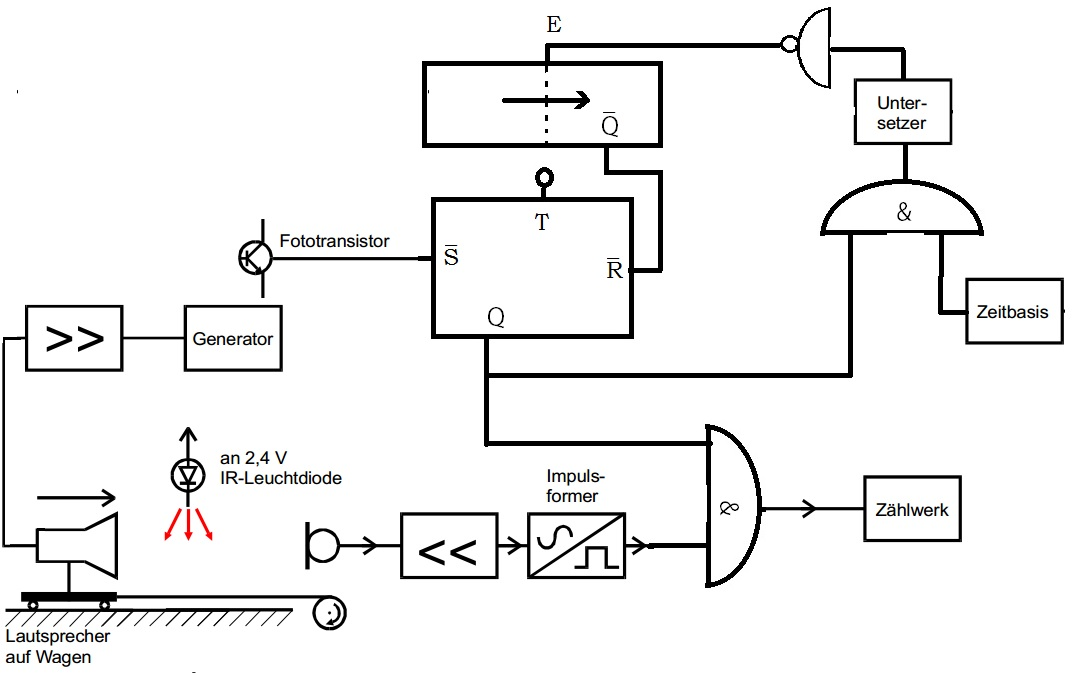
\includegraphics[scale=0.5]{Grafiken/V104_Abb3.jpg}
  \caption{Aufbau für die Messung der Frequenz (verändert aus \cite{V104})}
  \label{fig:V104_Abb3}
\end{figure}
\begin{figure}[!h]
  \centering
  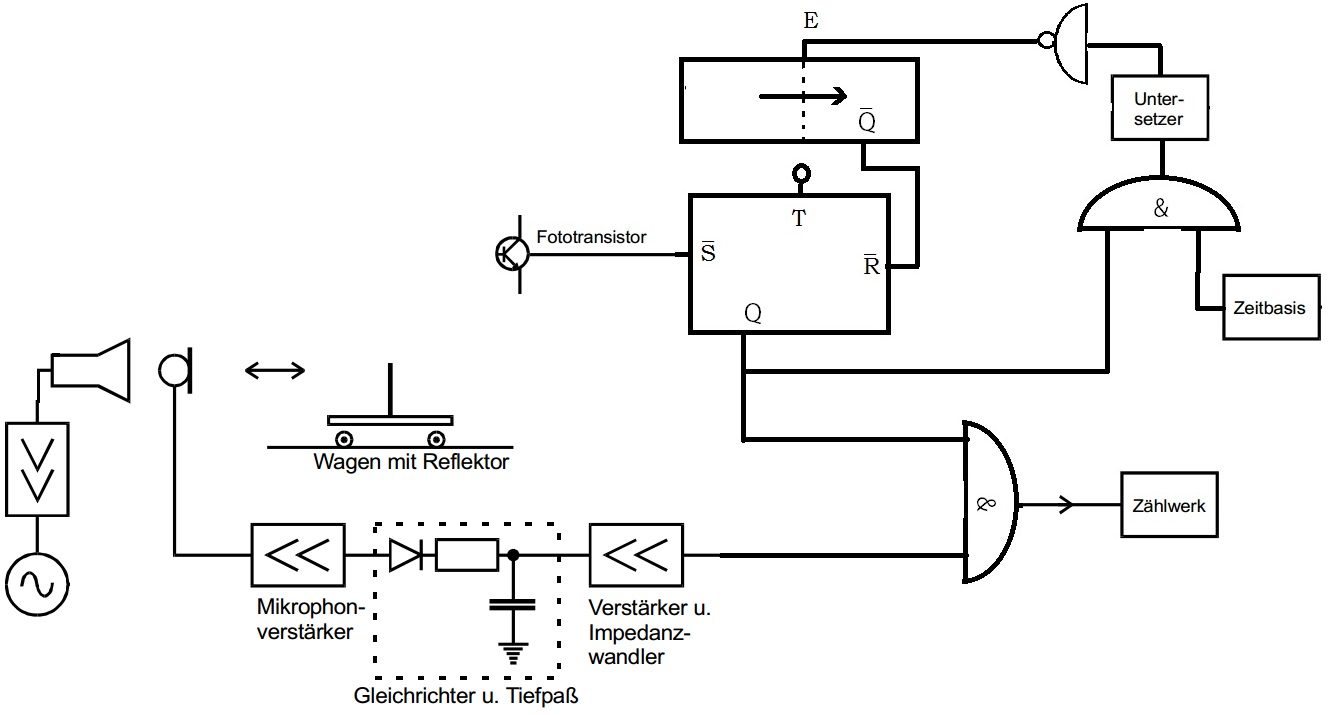
\includegraphics[scale=0.5]{Grafiken/V104_Abb4.jpg}
  \caption{Aufbau für die Messung der Frequenzdifferenz\\\hspace*{2.6cm} mittels Schwebung (verändert aus \cite{V104})}
  \label{fig:V104_Abb4}
\end{figure}

